\SourcePage{GELFAND-P000471}{unlabelled}
\uline{Lemma}. Let $f;g\colon K\longrightarrow K'$ be two morphisms.
\Unclear{GELFAND-P000471}{lemma-delimiter}{Two strokes appear between $f$ and $g$, here set as a semicolon.}
\end{GelfandAdjacentEvidence}
\begin{GelfandAdjacentEvidence}{GELFAND-P000471}{2}


The following statements are equivalent:

$1^\circ$. $\exists K_1$, $s_1\in S$:
\SourceFigure{GELFAND-P000471}{lemma-precomposition}{The first diagram with the equality written below it.\par\smallskip\centering
\begingroup\color{black}\GelfandFitDiagram{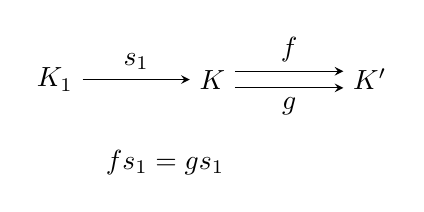
\begin{tikzpicture}[>=stealth]
\node (start) at (0,0) {$K_1$};
\node (middle) at (2,0) {$K$};
\node (end) at (4,0) {$K'$};
\draw[->] (start) -- node[above] {$s_1$} (middle);
\draw[->] ([yshift=3pt]middle.east) -- node[above] {$f$} ([yshift=3pt]end.west);
\draw[->] ([yshift=-3pt]middle.east) -- node[below] {$g$} ([yshift=-3pt]end.west);
\node at (1.4,-1.05) {$fs_1=gs_1$};
\end{tikzpicture}}\endgroup}
\end{GelfandAdjacentEvidence}
\begin{GelfandAdjacentEvidence}{GELFAND-P000471}{3}


$2^\circ$. $\exists K_2$, $s_2\in S$
\SourceFigure{GELFAND-P000471}{lemma-postcomposition}{The second diagram with the equality written below it.\par\smallskip\centering
\begingroup\color{black}\GelfandFitDiagram{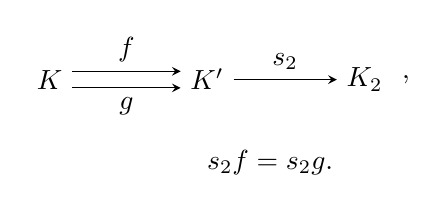
\begin{tikzpicture}[>=stealth]
\node (start) at (0,0) {$K$};
\node (middle) at (2,0) {$K'$};
\node (end) at (4,0) {$K_2$};
\draw[->] ([yshift=3pt]start.east) -- node[above] {$f$} ([yshift=3pt]middle.west);
\draw[->] ([yshift=-3pt]start.east) -- node[below] {$g$} ([yshift=-3pt]middle.west);
\draw[->] (middle) -- node[above] {$s_2$} (end);
\node[right] at (end.east) {,};
\node at (2.8,-1.05) {$s_2f=s_2g$.};
\end{tikzpicture}}\endgroup}
\end{GelfandAdjacentEvidence}
\begin{GelfandAdjacentEvidence}{GELFAND-P000471}{4}


{\centering\rule{3em}{.4pt}\quad\textperiodcentered\quad\rule{3.4em}{.4pt}\par}
$L_C$ — the same objects, and the morphisms: \uline{allow inverting \mbox{$s^{-1}$} and}
\par\hspace*{3em}\uline{Ore relations.}
\SourceFigure{GELFAND-P000471}{ore-insertion}{“Ore relations” is written below the first line, with a stepped rule.}
\end{GelfandAdjacentEvidence}
\begin{GelfandAdjacentEvidence}{GELFAND-P000471}{5}

The lemma makes it poss. to define the product correctly.
\Unclear{GELFAND-P000471}{product-reading}{The manuscript has «возможно» immediately before «корректно».}
\end{GelfandAdjacentEvidence}
\begin{GelfandAdjacentEvidence}{GELFAND-P000471}{6}


{\centering\rule{3em}{.4pt}\quad\textperiodcentered\quad\rule{3.5em}{.4pt}\par}
\(\overset{\scriptstyle +}{\text{See}}\)\quad\uline{Hartshorne}. Residues and duality.
\Unclear{GELFAND-P000471}{middle-reference-mark}{A short cross-shaped mark appears above «См.» (“See”).}
\end{GelfandAdjacentEvidence}
\begin{GelfandAdjacentEvidence}{GELFAND-P000471}{7}


{\centering\rule{3.9em}{.4pt}\quad\textperiodcentered\quad\rule{3.4em}{.4pt}\par}
\uuline{V. Buchstaber.}

\begin{tabular}{@{}llll@{}}
References: & C.–E. & 213--223 & (Cartan and Eilenberg)\\
 & M. & 358--370 & (Mac Lane)\\
 & Adams & Mat. $3\colon4$ & pp. 7--19.
\end{tabular}
\Unclear{GELFAND-P000471}{middle-maclane}{The parenthesis reads «Маклейн» (“Mac Lane”).}
\end{GelfandAdjacentEvidence}
\begin{GelfandAdjacentEvidence}{GELFAND-P000471}{8}


{\centering\rule{2.8em}{.4pt}\quad\textperiodcentered\quad\rule{3em}{.4pt}\par}
\[
A=\sum_{n\geqslant0}A_n\qquad\text{— grad. ring.}
\]
$A_n$ — an $A_0$-module for every $n\geqslant0$.
\[
0\longleftarrow A_0\xleftarrow{\varepsilon}A
\longleftarrow C_1\longleftarrow C_2\longleftarrow\cdots
\longleftarrow C_s\xleftarrow{d_{s+1}}C_{s+1}\longleftarrow\cdots
\]
($\varepsilon$ assigns $A$ zeroth comp. to each $a\in A$).
\Unclear{GELFAND-P000471}{lower-augmentation-a}{A separate $A$ is written immediately after «сопост.» (“assigns”).}
\end{GelfandAdjacentEvidence}
\begin{GelfandAdjacentEvidence}{GELFAND-P000471}{9}


Complete to a \uwave{grad. free resolution}.

The functor $\operatorname{Hom}_A(\cdot,A_0)$. takes $d_s$ to $(d_s)^*$.
\Unclear{GELFAND-P000471}{lower-hom-coefficient}{A small zero is visible below and to the right of the second argument $A$, against the parenthesis.}
\end{GelfandAdjacentEvidence}
\begin{GelfandAdjacentEvidence}{GELFAND-P000471}{10}

\[
H^s(A)=\operatorname{Ker}(d_{s+1})^*/\operatorname{Im}(d_s)^*
\]
\SourceFigure{GELFAND-P000471}{cohomology-index}{The numerator has $d_{s+1}$ and the denominator $d_s$.}
\end{GelfandAdjacentEvidence}


\uline{Theorem:}\quad 1) A free resolution exists

\hspace*{6em}2) The groups $H^s(A)$ are independent of the resolution.

\[
H(A)=\sum_{s=0}^{\infty}H^s(A)\qquad\text{— a graded ring.}
\]
A def. will be given for the multiplication of \uline{Yoneda}.
\[
\begin{gathered}
f\in H^i(A),\quad g\in H^j(A),\quad fg\in H^{i+j}(A),\\
\widetilde f\colon C_i\longrightarrow A_0;\qquad
\widetilde g\colon C_j\longrightarrow A_0.
\end{gathered}
\]


\Needspace{7\baselineskip}
\begin{GelfandAdjacentEvidence}{GELFAND-P000472}{1}
